\chapter{VAE Vizualizátor}
\label{vae}

V dnešnej dobe existujú dva spôsoby ako generovať obrázky pomocou neurónových sietí.
Z predchádzajúcich kapitol vieme, že ide o generatívne konkurenčné siete a variačné autoenkódery.
GAN implementáciu vizualizátora sme už ukázali, v tejto časti vysvetlíme ako sme postupovali v riešení nášho zadania využitím druhej zo spomínaných metód.

\section{Návrh}
Už vieme, že VAE generuje dáta z latentnej premennej.
Cieľom je preto namodelovať dáta \(X\) z rozdelenia pravdepodobnosti \(P(X)\).
Vzťah medzi latentnou premennou \(z\) a pravdepodobnosťou \(P(X)\) môžeme vyjadriť ako: \[P(X) = \int P(X|z)P(z)dz\]
Celou myšlienkou VAE je získať \(P(z)\) za pomoci \(P(z|X)\).
No nakoľko nepoznáme distribúciu \(P(z|X)\) využijeme jednoduchšie Gaussovo rozdelenie a minimalizujeme rozdiel medzi nimi využitím Kullback-Leiber divergencie.

Celkovú úlohu variačného autoenkódera môžeme zapísať takto: \[\log P(X) - D_{KL}[Q(z|X)||P(z|X)] = E[\log P(X|z)] - D_{KL} [Q(z|X)||P(z)]\]
To znamená, že chceme optimalizovať logaritmickú pravdepodobnosť dát \(P(X)\) so započítaním nejakej chyby.
Všimnime si, že čo v skutočnosti dostávame je \(P(X|z)\), čo generuje dáta so zohľadnením latentnej premennej, a \(Q(z|X)\), čo kóduje naše dáta do priestoru latentných premenných.

Toto všetko nám pomôže pri implementácii, no tento variačný autoenkóder nijako neumožňuje ovplyvniť výstup.
Kódovacia časť \(Q(z|X)\) ako aj dekódovacia časť \(P(X|z)\) modelujú výstup priamo zo vstupu a nezohľadňujú rôzne typy vstupov.
Tento problém vyriešime pridaním nového vstupu do oboch častí autoenkódera a dostávame tak \(P(X|z,c)\) a \(Q(z|X,c)\) čo pozmení úlohu na:
\[\log P(X|c) - D_{KL}[Q(z|X,c)||P(z|X,c)] = E[\log P(X|z,c)] - D_{KL} [Q(z|X,c)||P(z|c)]\]

Návrh modelu tejto neurónovej siete má dva časti.
\(P(X|z,c)\) je podsieť tvorená dvoma vrstvami.
Vstupná vrstva ma 128 neurónov, pričom každý má 649 vstupných kanálov.
549 vstupov tvoria hudobné akustické vlastnosti.
Ostávajúcich 100 vstupov zaberá vektor latentných premenných.
Výstupná vrstva generuje obrázky, preto počet jej neurónov zodpovedá rozmerom \(64\times64 = 4096\).
Podsieť \(Q(z|X,c)\) má na vstupnej vrstve, so 128 neurónmi, 4196 vstupov.
Ide od spojenie latentného vektora a obrázkov z datasetu.
Produkuje dva výstupy.
Každý o veľkosti 100.
Tieto sa neskôr spoja do jediného vektora \(z\), čo nám pomôže pri počítaní straty.

\section{Implementácia}
Definujme obe časti, opísané v návrhu.

\begin{minted}{python}
def P(z, c):
    inputs = tf.concat(axis=1, values=[z, c])
    h = tf.nn.relu(tf.matmul(inputs, P_W1) + P_b1)
    logits = tf.matmul(h, P_W2) + P_b2
    prob = tf.nn.sigmoid(logits)
    return prob, logits

def Q(X, c):
    inputs = tf.concat(axis=1, values=[X, c])
    h = tf.nn.relu(tf.matmul(inputs, Q_W1) + Q_b1)
    z_mu = tf.matmul(h, Q_W2_mu) + Q_b2_mu
    z_logvar = tf.matmul(h, Q_W2_sigma) + Q_b2_sigma
    return z_mu, z_logvar
\end{minted}

Aktivačnou funkciou vstupných vrstiev oboch častí je ReLu.
Rozdiel v kódery a dekódery je vidno na výstupe.
\(P(z, c)\) má na výstupe Sigmoid funkciu, nakoľko jednotlivé pixle majú hodnoty v rozmedzí 0 až 1.
\(Q(X, c)\) výstupnú aktivačnú funkciu nepotrebuje.
Ako sme vysvetlili v teoretickej časti práce, pri kódovaní vytvárame dva vektory.
Vektor \(z\_mu\) je vektor stredných hodnôt a vektor \(z\_logvar\) určuje disperziu.

Rozoberme si celkovú úlohu VAE siete.
Úlohou je maximalizovať pravdepodobnosť mapovania latentnej premennej na dáta a minimalizovať rozdiel medzi jednoduchou distribúciou \(Q(z|X,c)\) a skutočnou distribúciou \(P(z|c)\).
Maximalizácia \(E[\log P(X|z,c)]\) je v podstate odhad maximálnej pravdepodobnosti.
Práve preto je \(P(z, c)\) implementované ako klasifikátor a pre výpočet chyby môžeme využiť napríklad krížovú entropiu.
Pri druhej časti úlohy musíme myslieť na to, že chceme neskôr nejako zvoliť \(P(z|c)\).
Najjednoduchším spôsobom je brať vzorky z normálneho rozdelenia \(N(0,1)\).
Takže chceme aby rozdelenie \(Q(z|X,c)\) bolo čo najpodobnejšie \(N(0,1)\).
Zvoľme nech \(Q(z|X,c)\) je takisto Gaussovo normálne rozdelenie ale s priemerom rovným \(\mu(X)\) a disperziou \(\sum (X)\), čiže \(N(\mu(X), \sum (X))\).
Potom platí \[D_{KL}[N(\mu(X), \sum (X))||N(0,1)] = \frac{1}{2}  \sum_{k} (\sum (X) + \mu^{2} (X) - 1 - \log \sum (X))\]
Prakticky je ale stabilnejšie robiť \(\sum (X)\) namiesto \(\log \sum (X)\).
Náš finálny vzorec je \[D_{KL}[N(\mu(X), \sum (X))||N(0,1)] = \frac{1}{2}  \sum_{k} (exp(\sum (X)) + \mu^{2} (X) - 1 - \sum (X))\]

V kóde krížovú entropiu vypočítame za pomoci skutočných dát z datasetu.
Pre druhú časť chyby, do vzorca vložíme vektory \(z\_mu\) a \(z\_logvar\).
Celkovú chybu tvoria obe časti.
Pre optimalizáciu váh neurónovej siete využijeme Adam optimalizátor, ktorý sa snaží minimalizovať celkovú chybu.
\begin{minted}{python}
z_mu, z_logvar = Q(X, c)
z_sample = sample_z(z_mu, z_logvar)
_, logits = P(z_sample, c)

# Sampling from random z
X_samples, _ = P(z, c)
# E[log P(X|z,c)]
recon_loss = tf.reduce_sum(
	tf.nn.sigmoid_cross_entropy_with_logits(
		logits=logits, labels=X), 1)
# D_KL(Q(z|X,c) || P(z|c))
kl_loss = 0.5 * tf.reduce_sum(
	tf.exp(z_logvar) + z_mu**2 - 1. - z_logvar, 1)

vae_loss = tf.reduce_mean(recon_loss + kl_loss)
solver = tf.train.AdamOptimizer().minimize(vae_loss)
\end{minted}

\section{Trénovanie}
Trénovanie neurónových sietí môže byť zdĺhavý proces, pri ktorom jedinou technikou dosiahnutia výsledku je pokus-omyl.
Pre dosiahnutie vyhovujúcich zobrazení sme vyskúšali niekoľko rôznych konfigurácií systému.
Už pri trénovaní pôvodného návrhu sme spozorovali, rýchle rozloženie datasetu do priestoru normálneho rozdelenia.
Ako sa ale dalo čakať, tento model nebol dostatočne komplexný aby vykreslil správny typ obrázkov.
Pôvodne sme predpokladali, že problém môže byť v počte rozmerov vektora \(z\).
Zmenili sme teda \(|z|\) zo 100 na 1000 a nechali spustené trénovanie niekoľko hodín.
Výsledky boli takmer totožné.
V obidvoch prípadoch sieť dokázala vykresliť vzorky datasetu so 100\% presnosťou no pri vložení nových skladieb na vstup, vytvorené obrázky obsahovali len šum bez obsahu.

Skôr ako sme pristúpili k zmenám v typológií siete, otestovali sme inú štruktúru datasetu.
Namiesto pôvodných 549 hudobných vlastností, pri ďalšom trénovaní do siete vstupovali len miery nulových prechodov a tempo, čiže 28 čísel z oboru reálnych hodnôt.
Opäť sme vyskúšali varianty s malým aj veľkým latentným vektorom.
Obrázky vygenerované, v tomto pokuse takisto neboli v dostačujúcej kvalite, no pri niektorých skladbách sme spozorovali náznaky obsahu.
Takisto bolo zjavné, že pri \(|z| = 1000\) sa lepšie výsledky objavovali častejšie.

Ďalším krokom bolo pozmeniť sieť ako takú.
Pridali sme do kódovacej aj dekódovacej časti siete zhodne po dvoch skrytých vrstvách.
Každá obsahovala 128 neurónov s aktivačnou funkciou ReLu.
Trénovanie bolo konečne úspešné.
Pri každej testovacej skladbe aspoň jeden zo šestnástich vygenerovaných obrázkov mal viditeľný obsah.
Takisto sa potvrdilo, že je lepšie nastaviť počet rozmerov latentného vektora na 1000, nakoľko obrázky v tomto prípade boli kvalitnejšie.

Tento úspech nás priviedol k myšlienke, že počiatočné neúspechy nesúviseli so štruktúrou vstupných dát.
Otestovali sme teda novú sieť aj pre pôvodný dataset.
Trénovanie potvrdilo túto skutočnosť, čo naznačovalo, že problém v kvalite výstupov zapríčiňuje \(P(X|z,c)\) časť problému.
Rozhodli sme sa ďalej zväčšiť \(P(z, c)\) sieť o dve nové skryté vrstvy, totožné s už existujúcimi skrytými vrstvami.
Nová konfigurácia modelu generovala kvalitné výstupy.

Už len pre kontrolu sme zmenšili \(P\) aj \(Q\) o jednu vrstvu.
Nespozorovali sme žiadny nárast vo variabilite výstupu, naopak kvalita obrázkov sa zhoršila.
Teda môžeme povedať, že predchádzajúci model je dostatočným riešením.

Vytrénovali sme ešte raz tento model ale na dátach so zmenšeným oborom akustických hodnôt.
V porovnaní s pôvodným datasetom takto vytrénovaný variačný autoenkóder produkoval rôznorodejšie obrázky.
Tento výsledok sa dal čakať nakoľko rozdiel v počte nulových prechodov a tempe v dvoch rozdielnych skladbách nemusí byť dostatočným meradlom.

Takisto sa tento model ukázal byť vhodným aj pri generovaný farebných detailných obrázkov.
Jedinou zmenou v sieti, je zväčšenie vstupu \(Q\) siete a výstupu \(P\) siete.
Ide o to, že skice v datasete majú každý pixel uložený ako jednotku alebo nulu.
Pri farebných obrázkoch je každý pixel reprezentovaný tromi číslami.
Čiže tieto vstupné respektíve výstupne vrstvy namiesto 4096 neurónov obsahujú \(4096 \times 3 = 12288\) neurónov.
Nakoľko sieť tak obsahuje väčšie vrstvy, čas jednej epochy pri trénovaní sa približne strojnásobil.
\begin{figure}[!t] 
	\centering 
	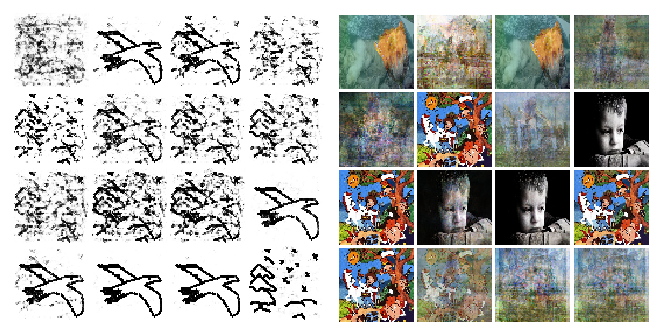
\includegraphics[width=.8\textwidth]{figures/vae_mozart} 
	\caption{Výstup variačného autoenkódera pri Mozartovej skladbe Turkish March} 
	\label{vae_mozart}
\end{figure}
Príkladom výstupu je obrázok \ref{vae_mozart}.
Vľavo je výstup vygenerovaný modelom, ktorý sa učil z datasetu skíc.
Vpravo bol použitý dataset farebných obrázkov.
Obe výstupy zobrazujú skladbu Turkish March od Mozarta, pričom ide o 16 dvadsaťpäť sekundových úsekov, ktorých odstup je jedna sekunda.
